\documentclass[12pt]{article}
\usepackage[utf8]{inputenc}
\usepackage[a4paper,top=2.5cm,bottom=2.5cm,left=2cm,right=2cm]{geometry}
\usepackage{amsmath}
%\usepackage{upgreek}
\usepackage{enumerate}
\usepackage{indentfirst}
\usepackage{subcaption}
\usepackage{graphicx}
%\usepackage{caption}
% This line is what's in the Lab on a Chip template, and what we need to correct for subfigures
\usepackage[format=plain,justification=raggedright,singlelinecheck=false,font={small,sf},labelfont=bf,labelsep=space]{caption}
% And this is how we correct it
\captionsetup[subfigure]{labelfont=sf,justification=centering}
\usepackage{siunitx}
\usepackage{array}
\usepackage{multirow}

\setlength{\parindent}{4ex}

\title{Test doing multi-part figure with subcaption package}
\author{author's name}
\date{}

% subcaption package instructions: http://texdoc.net/texmf-dist/doc/latex/caption/subcaption.pdf
% how to format subfigure captions: http://www.peteryu.ca/tutorials/publishing/latex_captions

%-----------------------------------------------
\begin{document}
\maketitle

\noindent Let's include two figures.

\begin{figure}[h]
\centering
\begin{subfigure} {0.5\textwidth}
  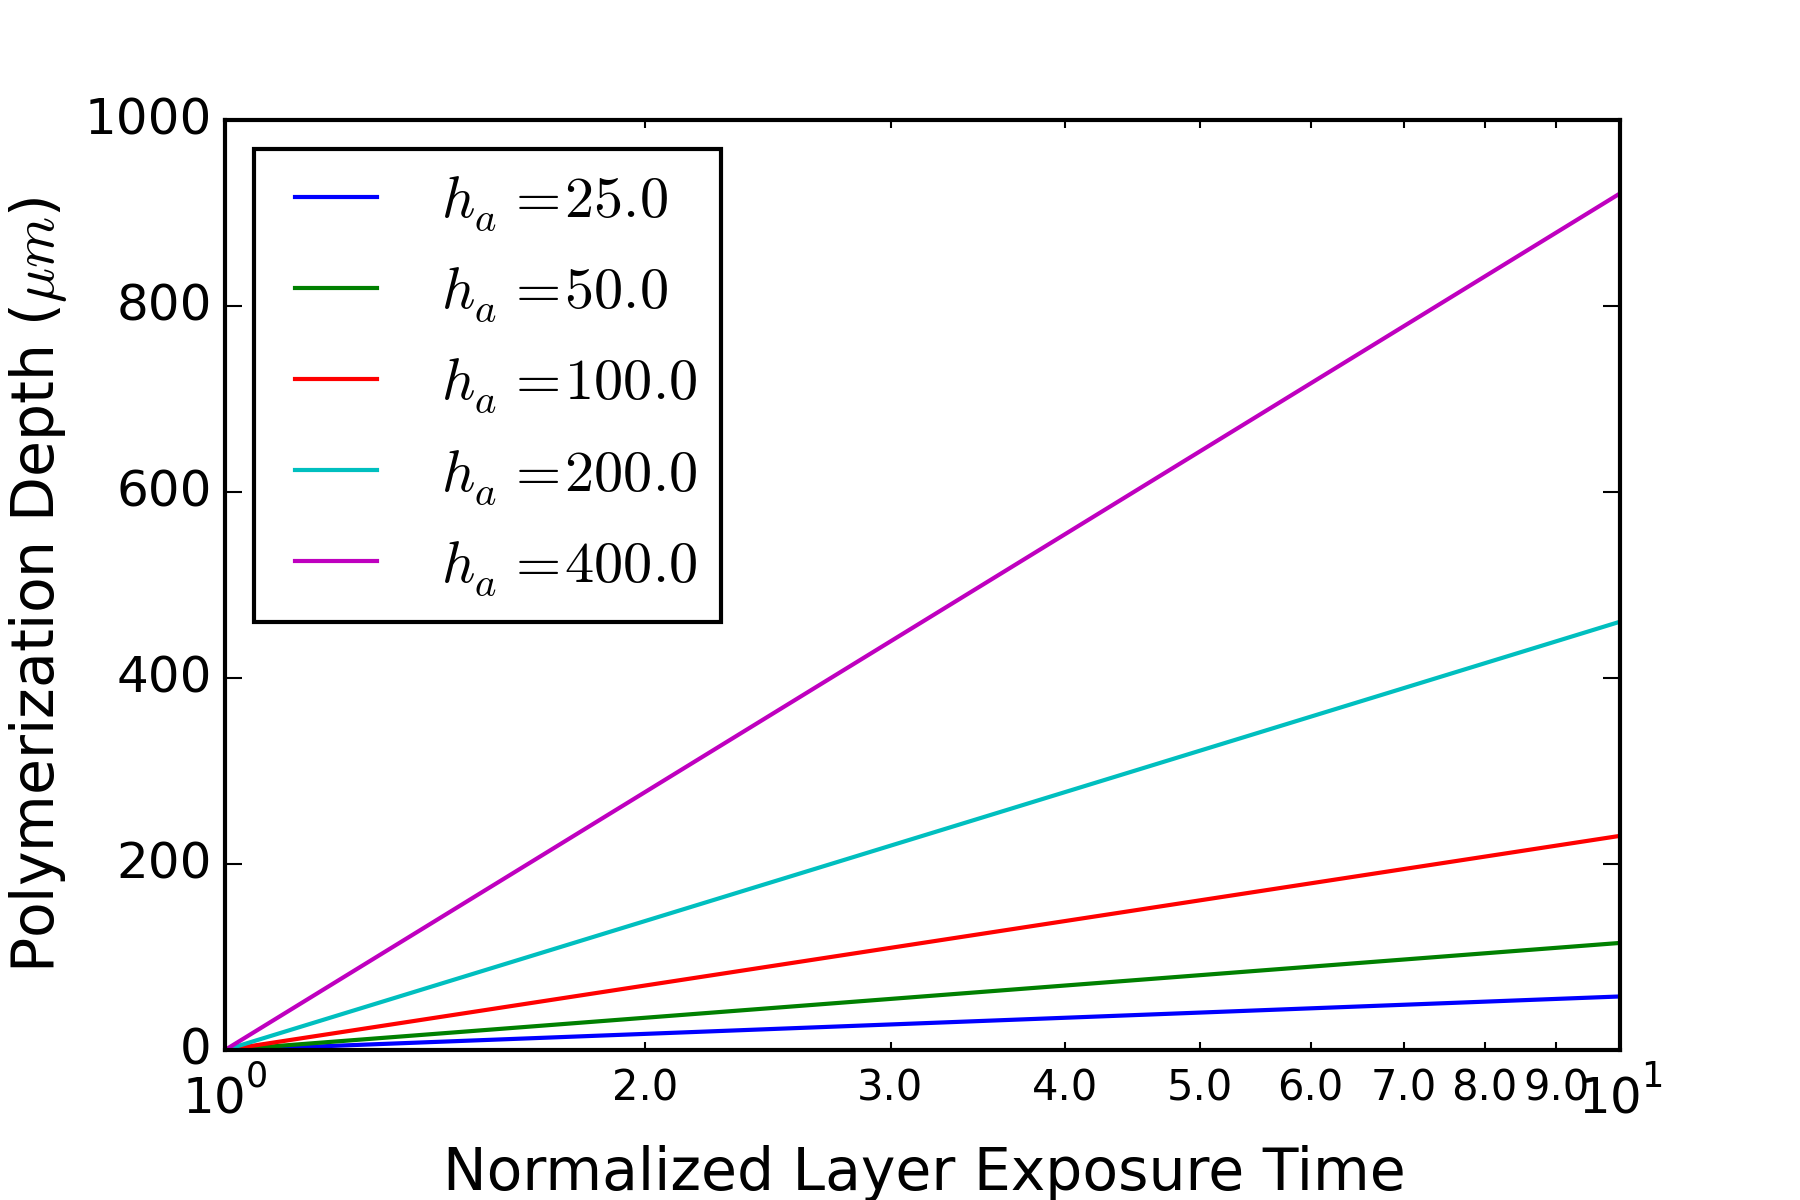
\includegraphics[width=\linewidth]{figures/beerslaw1.png}
   \caption{HELP!} \label{fgr:beerslaw1}
\end{subfigure}
\begin{subfigure} {0.5\textwidth}
  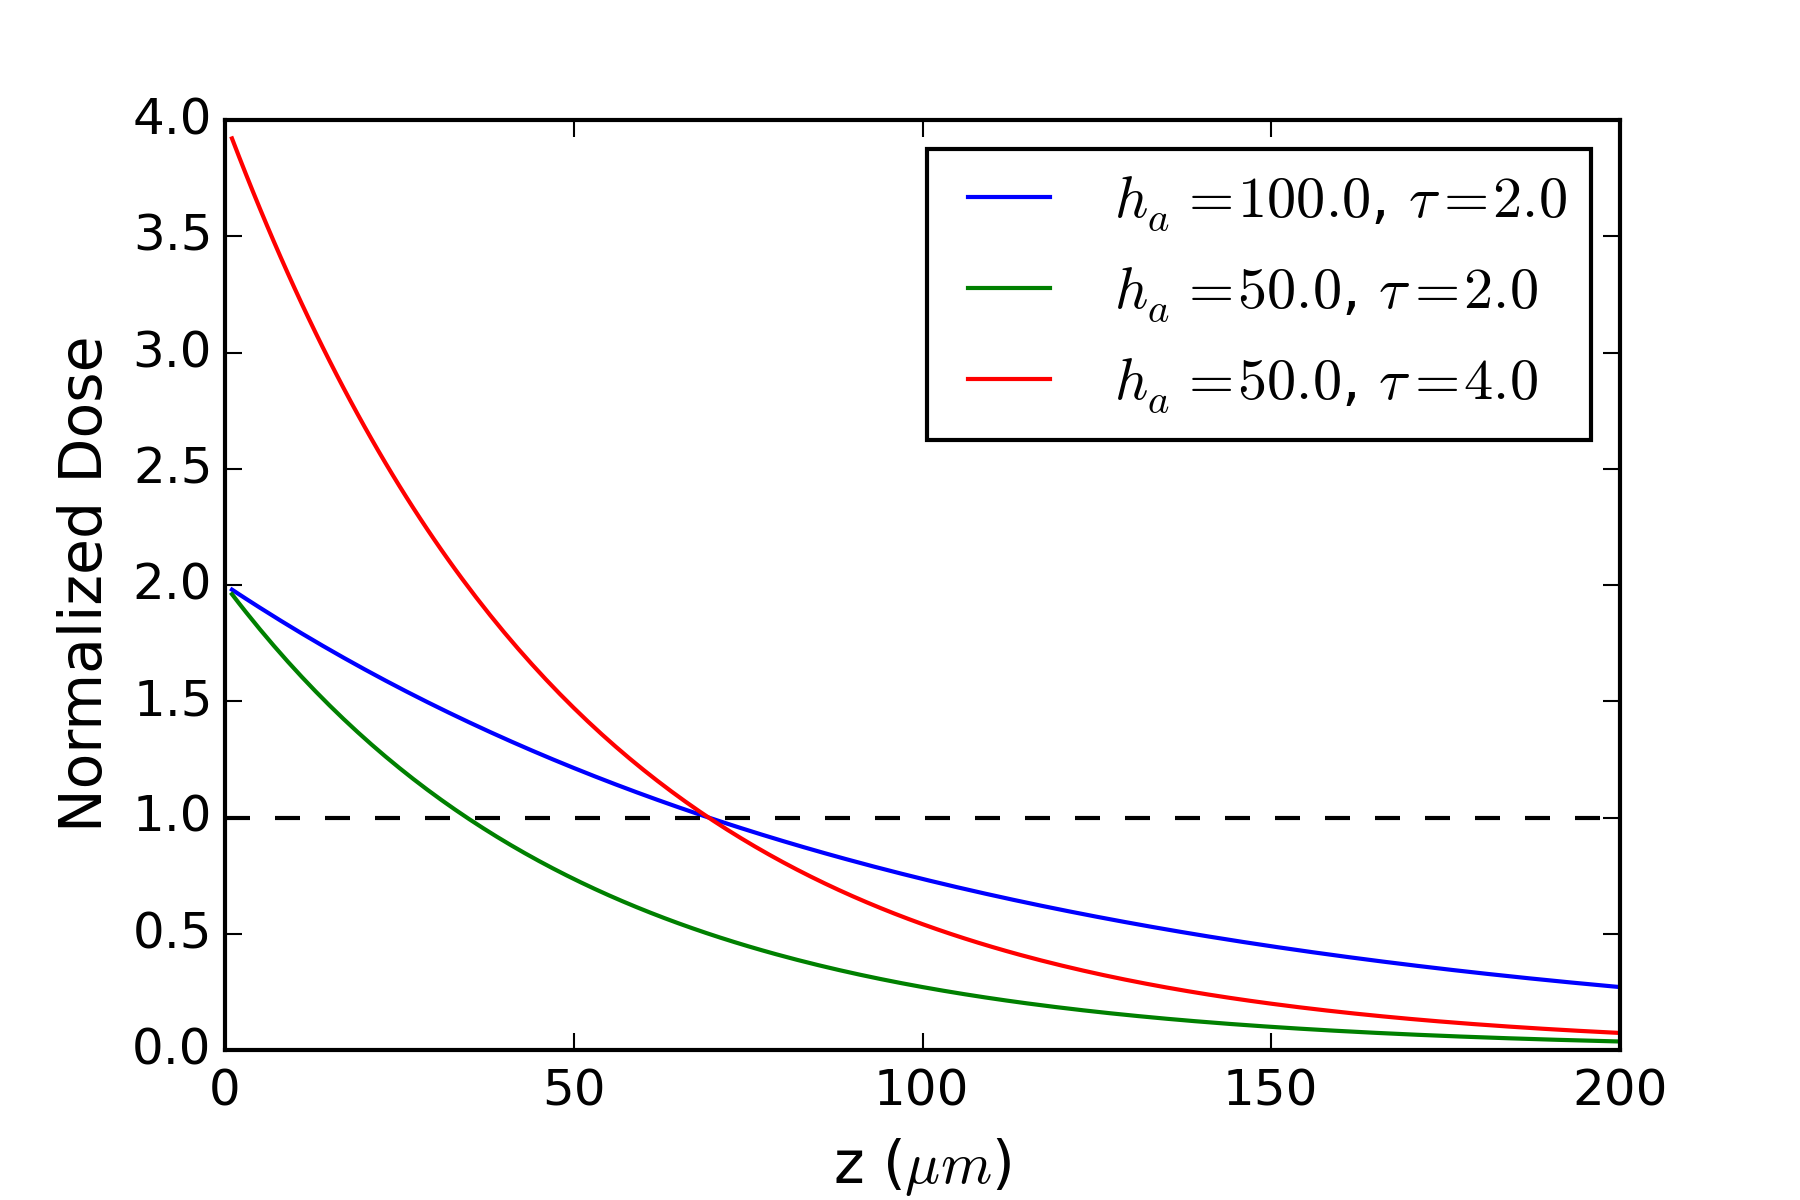
\includegraphics[width=\linewidth]{figures/beerslaw2.png}
   \caption{} \label{fgr:beerslaw2}
\end{subfigure}
\caption{(a) Polymerization depth of resins with different $h_a$ vs. normalized layer exposure time. (b) Polymerization depth of the same resin with different normalized dose, and one same dose for a different resin.}
\end{figure}

some text. some more text. \ref{fgr:beerslaw1}

\noindent And now we'll reference them as Fig. \ref{fgr:beerslaw1} and Fig. \ref{fgr:beerslaw2}.


\end{document}